\documentclass[]{article}
\usepackage{hyperref}
\usepackage{amsmath}
\usepackage[margin=1.5in]{geometry}
\usepackage[utf8]{inputenc}
\usepackage[parfill]{parskip}
\usepackage[english]{babel}
\usepackage[autostyle]{csquotes}
\usepackage[style=numeric,backend=biber]{biblatex}
\usepackage[pdftex]{graphicx} % Image import.
\usepackage{pgfplots}
\usepackage{float}

\addbibresource{biblio.bib}

\newcommand{\clique}{\textsc{clique}}
\newcommand{\sat}{\textsc{sat}}

%opening
\title{Approaching the Clique Problem\\ With SAT Solvers\\[.2cm]
	\large{CIS 673: Computer Aided Verification}}
\author{Matthew Howard}

\begin{document}
	
	\maketitle
	
	\begin{abstract}
		Modern SAT solvers are able to solve real world instances of \textsc{sat} within realistic time and space restrictions. General purpose solvers have been effective in solving artificial intelligence problems, circuit optimizations, logic puzzles, and verification problems. In this project, we evaluate the application of a SAT solver to the classical graph theoretic \clique{} problem.
	\end{abstract}
	
	\section{The Clique Problem}
	
	Let us start by defining terminology. A \textit{graph} is a duple $G = (V, E)$ consisting of a vertex set $V$ and an edge set $E \subseteq \{(u, v) ~\vert~ u, v \in~V, u \neq v\}$. We will follow the convention $n = |V|$ and $m = |E|$. An \textit{induced subgraph} $G' = (V', E')$ of $G$ consists of a vertex set $V' \subseteq V$ and the maximal edge subset $E' \subseteq E$ such that the endpoints of each edge are in $V'$, formally $E' = \{(u, v) \in E ~\vert~ u, v \in V'\}$. For the purpose of this project1, we are concerned only with undirected, unweighted graphs.
	
	A graph is \textit{complete} if there exists an edge between every two distinct vertices.
	
	A \textit{clique} $G' = (V', E')$ in $G$ is an induced subgraph which is also a complete graph. We say a clique is of size $k$ if its vertex set contains $k$ elements. The \textit{Clique Problem}, which we refer to as \clique{}, is the problem of determining for a graph $G$ and a positive integer $k$ whether there exists an induced subgraph $G'$ satisfying the following two conditions:
	\begin{enumerate}
		\item \textbf{(Clique Condition)} $G'$ is a clique in $G$
		\item \textbf{(Size Condition)} $G'$ is of size at least $k$
	\end{enumerate}	
	
	Note that for a clique $G'$ in $G$, every induced subgraph $G''$ of $G'$ is also a clique in $G$, so we could equivalently formulate \clique{} with the more strict size condition ``$G'$ is of size exactly $k$''.
	
	While we are concerned mostly with the decision problem formulation of \clique{}, it's worth discussing the closely related optimization version: Given a graph $G'$, find a clique of maximum size. We define $\omega(G)$ to be the maximum clique size of a graph $G$. The optimization and decision versions are similar in complexity. If $\omega(G)$ is known, then the decision problem is equivalent to checking if $k \le \omega(G)$. Likewise, if we have an oracle for \clique{} which provides the clique's vertex set as a certificate, then we can solve the optimization version in $O(\log n)$ calls to the oracle with a binary search of $k$.
	
	The clique problem is of significance in complexity theory for a few reasons. Firstly, it is one of the classical NP-complete problems. \clique{} is in NP since the vertex set of a $k$ clique can serve as a $O(n)$ certificate from which it is easy to verify the Clique and Size properties. \clique{} can be shown to be NP-hard through the two reductions,
	\begin{align}
	\textsc{sat} \le_p \textsc{3sat} \le_p \clique
	\end{align}
	
	Secondly, the hardness of \clique{} is often exploited in proving the NP-hardness of \textsc{vertex-cover} and other NP-hard problems which indicates it is a powerful and useful problem. Finally, \clique{} is ``hard'' in the algorithmic sense that there does not exist an approximation algorithm which performs better than $n^{1 - \epsilon}$\cite{Hastad1999}. This hardness of approximation sets \clique{} apart from many other classical NP-complete problems.
	
	\section{Selection of a SAT Solver}
	Rather than performing a survey of different SAT solvers (which is already done each year on a global scale), we chose to focus our efforts one solver in particular. MiniSat is widely used, open source, minimalistic, and designed for integration, which makes it an good candidate to serve as the foundation for our \clique{} solver. MiniSat works through conflict-driven learning and unit propagation{Een03anextensible}.
	
	\section{Obtaining Data Sets}
	We want to analyze our clique solver on both real-world and randomly-generated graphs. We decide to go with Facebook friend networks as our source of real data. Vertices correspond to friends of a central user (without including the central user as a vertex) and edges correspond to friendships between users in the graph. A clique is intuitively a group of people who are all friends with each other. Running analyses on real data allows us to draw social insights from our application. For example, given a large clique, we can identify common traits between the constituents, such as membership in a club or a certain place of employment.
	
	\subsection{Social Network Data}
	The Facebook Graph API provides REST access to the information we require, including lists of friends and lists of mutual friends in easily parsable formats. However, since the release of version 2.0 of the API, lists only show friends who have actively logged into the developer's particular application (in this case our data collection tool)\cite{facebook2014}. This severely restricts the usefulness of this data. One alternative approach to collecting the same data would be to write a web-scraper using a browser automation tool like Selenium. However, this solution begs complex ethical and legal implications since neither Facebook nor the users consent to this style of data collection.
	
	Luckily, the Stanford Network Analysis Project provides a handful of anonymized, real-world datasets including graphs of Facebook friend data. While the anonymous nature of this data limits social insights that could come out of our analysis, the datasets will nonetheless allow us to test our solvers on real-world data.
	
	The Stanford Datasets provides us with ten graphs of varying sizes. We label these graphs \texttt{facebook.a} through \texttt{facebook.j}.
	
	%\subsection{Random Datasets}
	%Since the Facebook datasets are limited in number and cannot be generated to be arbitrary large, we want another source of graph data. We wrote a script to generate a Erdős - Renyi graph (i.e. edges chosen uniformly at random) given values for $n$ and $m$. Then, we generated ten graphs with values of $n$ and $m$ matching those of the Facebook graphs. We label these \texttt{random.a} through \texttt{random.j}.
	
	%Since the probability of finding a large clique in a graph generated from this method is very low since the edges are spread uniformly among all node pairs and so high concentrations of edges within certain subgraphs are unlikely compared to in a social network graph, where they arise naturally. Since we want to test the upper limits of our solver, we want to produce arbitrarily large graphs with high clique numbers. A simple approach is to randomly generate a graph with different edge probabilities according to vertex groupings. Specifically, we want to 
	
	\subsection{Analyzing the Data}
	Before we run and evaluate our clique solver, we wish to analyze the graph datasets. We leverage ``igraph'', an open source graph analysis library with a Python wrapper to compute $\omega(G)$. igraph's $\omega(G)$ routine is based off of an algorithm due to Tsukiyama \textit{et al.}\cite{doi:10.1137/0206036} and has a worst-case runtime of $O\left(3^{n/3}\right)$\cite{igraph2016}. This implementation will serve as a point of comparison for the performance of our \clique{} solver.
	
	\section{Reduction Strategy}
	Given a graph $G$ and a positive integer $k$, we want to produce an instance of \sat{} such that the \sat{} system is satisfiable if and only if our graph contains a clique $G'$ of at least size $k$. Every \sat{} instance consists of variables and clauses. Since a clique is defined by its vertex set and a solution to \sat{} is defined by a set of variable assignments, we naturally correspond vertices to variables. For all $v \in V$, let $x_v$ represent the variable indicating whether $v \in V'$.
	 
	Given the vertices are represented by variables, we need some way of encoding edges in our \sat{} system. The Size Condition in \clique{} is independent of the edge set $E$ and only depends on the truth assignments of variables in the vertex set $V'$. Therefore, we must reference our edge set $E$ in terms of the Clique Condition.
	
	We restate our Clique Condition as:
	\begin{align}
	\forall~u,v \in V,&& \quad u \in V' \land v \in V' &\implies (u, v) \in E \\
	\forall~u,v \in V,&& x_u \land x_v &\implies (u, v) \in E
	\end{align}
	
	If we take the contrapositive, we get
	\begin{align}
	\forall~u,v \in V,&& (u, v) \notin E &\implies \lnot x_u \lor \lnot x_v \\
	\forall~u,v \in V,&& (u, v) \in \overline{E} &\implies \lnot x_u \lor \lnot x_v\\
	\forall~ (u, v) \in \overline{E},&& &\lnot x_u \lor \lnot x_v
	\end{align}
	where $\overline{E}$ is the complement edge set, or formally $\overline{E} = \{(u, v) ~\vert~ u, v \in V,~u \neq v\} \setminus E$. This last statement of the clique condition can easily be encoded in \sat{} since $\lnot x_u \lor \lnot x_v$ is a CNF clause and $\overline{E}$ is an enumerable set of size $O(n^2 - m)$ over which we can add clauses.
	
	The Size Condition is a bit trickier. We must add variables and clauses such that at least $k$ of our vertex variables must be true. If we number our vertices $1 \ldots n$ and consider our vertex variables as binary indicator variables, we want
	\begin{align}
	\sum_{i = 1}^{n} x_i \ge k
	\end{align}
	The computation on the left hand side can be represented as a combinational digital logic circuit with $n$ single-bit inputs and one $(\lfloor\log_2 n\rfloor + 1)$-bit output. Let us define $k'$ to be the least natural number such that $k + k'$ is a power of 2, say $2^p$. Adding $k'$ to both sides, we get 
	\begin{align}
	\sum_{i = 1}^{n} x_i + k' \ge k + k'
	\end{align}
	This expression is equivalent to checking whether the $p$-th bit of the sum on the left hand size is equal to 1, which can be expressed as a one-literal clause.
	
	We implement the sum using an adder tree. The leaves of the tree are the vertex variables and $k'$ while the internal nodes are binary adders of varying size. The $j$-bit binary adders are constructed from full adders, which are comprised of NAND and NOR gates, which are constructed from boolean clauses with additional variables.
	
		\begin{figure}[H]
			\caption{Adder Tree Schematic}
			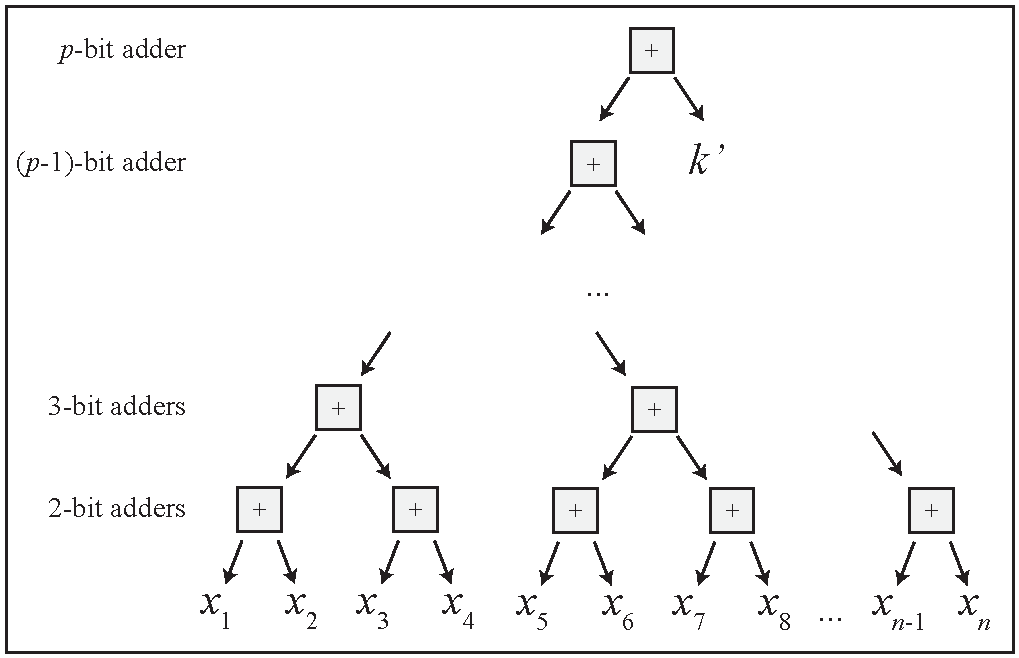
\includegraphics[width=4.5 in]{adder-tree}
			\centering
		\end{figure}

	We can run this reduction on the Facebook datasets with $k = \omega(G)$ to see the size of the resulting \sat{} systems.

	\begin{figure}[H]
		\centering
		\caption{Number of \sat{} Literals and Variables when $k = \omega(G)$}
		\begin{tabular}{|c|c|c|c|c|}
			\hline
			Name                & $n$  & $m$   & Variables & Literals \\ \hline
			\texttt{facebook.a} & 333  & 5038  & 2286      & 60199    \\ \hline
			\texttt{facebook.b} & 1034 & 53498 & 7193      & 531836   \\ \hline
			\texttt{facebook.c} & 224  & 6384  & 1559      & 26819    \\ \hline
			\texttt{facebook.d} & 150  & 3386  & 1041      & 12909    \\ \hline
			\texttt{facebook.e} & 168  & 3312  & 1154      & 16091    \\ \hline
			\texttt{facebook.f} & 61   & 540   & 424       & 2931     \\ \hline
			\texttt{facebook.g} & 786  & 28048 & 5457      & 312068   \\ \hline
			\texttt{facebook.h} & 747  & 60050 & 5220      & 265496   \\ \hline
			\texttt{facebook.i} & 534  & 9626  & 3644      & 149737   \\ \hline
			\texttt{facebook.j} & 52   & 292   & 355       & 2287     \\ \hline
		\end{tabular}
	\end{figure}
	
	While the adder tree introduces many additional variables and clauses, the set of added variables only has one satisfying assignment for each assignment of the vertex variables. MiniSat should be able to pick assignments to the vertex variables and then solve the intermediate variables in the adder tree via unit propagation\cite{matesoos}.

	\section{Evaluation}
	
	To test the correctness of our clique solver, we verify it produces the same values for $\omega(G)$ as the igraph script. A proof of $\omega(G)$ with our \clique{} solver consists of showing that the program succeeds when $k = \omega(G)$ and that the program fails when $k = \omega(G) + 1$,. In other words, there exists a clique of size $\omega(G)$ but no clique of size larger than $\omega(G)$. We first run our igraph script on each \texttt{Facebook} graph and get results for all values except \texttt{facebook.h}. igraph's $\omega$ function runs on \texttt{facebook.h} for at least 30 CPU minutes. Since this is far more than the computation time required for any of the other graphs, we classify igraph's $\omega$ algorithm as not terminating on \texttt{facebook.h} within a reasonable length of time.
	
	Next, we run our \clique{} solver on the same set of graphs for our previously obtained values of $\omega(G)$ and $\omega(G) + 1$. We compute $\omega(\texttt{facebook.h})$ using our solver in about 15 minutes.
	\begin{figure}[H]
		\centering
		\caption{igraph and \clique{} Solver Performance on Facebook Datasets}
		\label{facebooktimetable}
		\begin{tabular}{|c|c|c|c|r|r|r|}
			\hline
			\multicolumn{4}{|l|}{}            & igraph    & \multicolumn{2}{c|}{\clique{} Solver} \\ \hline
			Name       & n    & m     & $\omega$ & $\omega$ time    & $k = \omega$ time        & $k = (\omega + 1)$ time      \\ \hline \hline
			\texttt{facebook.a} & 333  & 5038  & 15    & 0.0156  & 0.141      & 0.594           \\ \hline
			\texttt{facebook.b} & 1034 & 53498 & 37    & 16.859 & 4.906       & 29.297           \\ \hline
			\texttt{facebook.c} & 224  & 6384  & 18    & 0.0625    & 0.141      & 0.359          \\ \hline
			\texttt{facebook.d} & 150  & 3386  & 18    & 0         & 0.0469      & 0.0938           \\ \hline
			\texttt{facebook.e} & 168  & 3312  & 16    & 0.0156  & 0.0313       & 0.0938           \\ \hline
			\texttt{facebook.f} & 61   & 540   & 10    & 0         & 0             & 0.0156          \\ \hline
			\texttt{facebook.g} & 786  & 28048 & 26    & 0.563    & 1.266       & 7.484           \\ \hline
			\texttt{facebook.h} & 747  & 60050 & 68    & -         & 12.813       & 694.594           \\ \hline
			\texttt{facebook.i} & 534  & 9626  & 16    & 0.0313   & 0.297      & 2.0938           \\ \hline
			\texttt{facebook.j} & 52   & 292   & 6     & 0         & 0.0156      & 0.0156          \\ \hline
		\end{tabular}
	\end{figure}
	
	For each graph, we plot the maximum clique size versus the execution time for igraph's $\omega$ calculation, for our solver with $k = \omega$, and for our solver with $k = (\omega + 1)$.
	
	\begin{figure}[H]
		\caption{Clique Size vs. Computation Time for Facebook Datasets}
		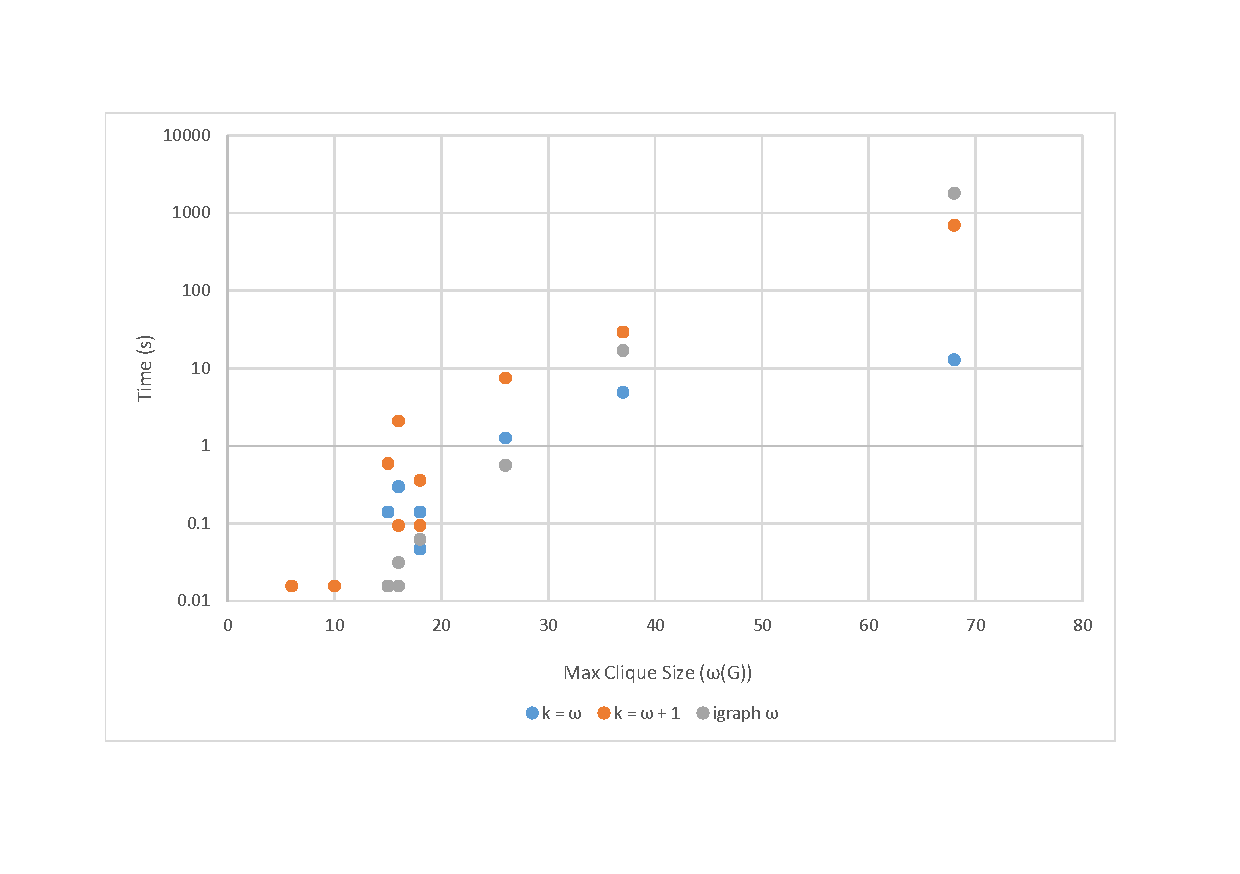
\includegraphics[width=4.5 in]{graph1}
		\centering
	\end{figure}
	
	From this small set of data, we see a rough exponential relationship between clique size and run time for both our solver and igraph. This is expected since both programs have exponential bounds.
	
	In addition to computation time, MiniSat keeps track of other useful metrics. By default, it reports the number of restarts, conflicts, decisions, propagations, and conflict literals at the end of execution. The number of conflicts in particular ends up being a fair indicator of problem complexity and is strongly associated with execution time. This figure is also telling of how MiniSat responds to a particular problem since the conflicts correspond to pieces of information MiniSat is able to learn as it progresses through its search.
	
	\subsection{Effects of $k$ on Runtime}
	We can see for a fixed graph what effect varying $k$ has on our solver's execution time. Intuitively, very small cliques, e.g. $k = 2$ or $k = 3$ should come up very quickly in the MiniSAT's search of the solution space, whereas finding cliques of size close to $\omega(G)$ should require more searching and time based on the hardness of the problem. We fix the graph \texttt{facebook.b}, which has one of the higher $\omega$ values ($\omega(G) = 37$) of our dataset. Then we run our solver three times for each value of $k$ between 1 and 50 and plot the results.
	
	\begin{figure}[H]
		\caption{$k$ vs. Computation Time}
		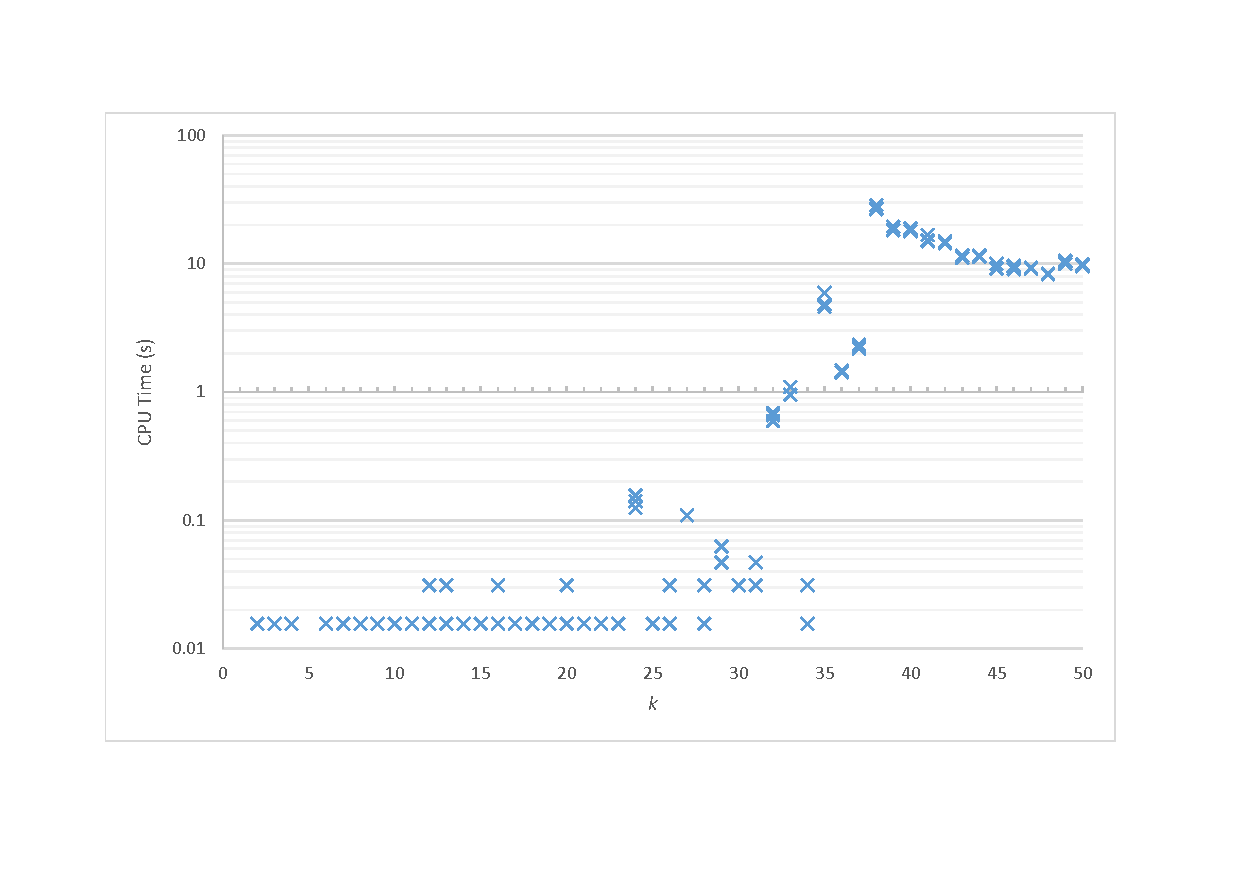
\includegraphics[width=4.5 in]{graph2}
		\centering
	\end{figure}
	
	We observe that for $k < 24$, the computation time stays at or around 0. For $24 \le k \le \omega = 37$, there is a positive association but the the CPU time does not increase monotonically as we increase k. For example, the average computation time for $k = 35$ is 5.125 seconds while the average computation time for $k = 36$ is 1.443 seconds, despite the fact that it is strictly more difficult to find a clique of size 36 than to find one of size 35. This insight, combined with the fact that there is little deviation in computation time across trials for a fixed $k$, suggests that the value of $k$, encoded in our reduction via $k'$ and the bit width of the adder tree root, plays a large role in guiding the behavior of MiniSat.
	
	Between $k = \omega = 37$ and $k = \omega + 1 = 38$, the average computation time jumps from 2.26 seconds to 27.4 seconds. This sudden increase between $\omega$ and $\omega + 1$ appears consistently in Figure \ref{facebooktimetable} as well. One possible reason is that when $k = \omega + 1$, there are many assignments which come close to satisfying the Size Condition, all of which must be ruled out in order to conclude no satisfying assignment exists.
	
	For $\omega + 1 = 38 \le k \le 50$, the computation time steadily decreases. This aligns with out intuition, because as $k > \omega$ increases, the number of possible satisfying assignments to check, $\binom{n}{k}$, decreases. By extension, the solver concludes that the system is unsatisfiable for $k = n = 1024$ in only 0.203 seconds.
	
	\section{Conclusion}
	In this project, we constructed a reduction for $\clique \le_p \sat$, implemented it in C++, interfaced our reduction with MiniSat, and then tested and evaluated the resulting \clique{} solver. Our construction operating on top of a general purpose \sat{} solver had comparable performance to igraph's specialized $\omega(G)$ routine. This speaks to the power and generality of MiniSat as a computational tool.
	
	Our analysis was heavily constrained by the availability of good graph data. We tried to construct random graphs using the Erdős - Renyi model but found that the uniform distribution of edges between pairs of vertices results in very small clique sizes, which limits the graphs' usefulness to our analysis. We also looked at a slightly more complex graph generation model consisting of vertex typing and type-wise connection probabilities. While graphs of this model yielded significantly larger clique sizes, they still failed to mimic the eccentricity distributions of social media graphs and were difficult to generate for varying parameters of $n$ and $m$.
	
	Given more time, we would have considered other graph generation models to aid in analysis. One family of graph models, the Kronecker Product Graph Model construction, has been very successful in mimicking social network graphs\cite{Leskovec:2010:KGA:1756006.1756039}, including Facebook friend graphs\cite{moreno2013block}. Given the ability to generate these social network graphs of arbitrary size, we could have further tested the limitations and runtime of our solver.
	
	\section{Resources}
	The code and data involved in this project is publicly available at \url{https://github.com/moward/CliqueSolver}.
	
	\printbibliography

\end{document}
